% !TEX root = epifanov_solid_state_physics.tex
%!TEX TS-program = pdflatex
%!TEX encoding = UTF-8 Unicode


\chapter[Mechanical Properties of Solids]{Mechanical Properties of Solids}\label{chap:2}
% \chaptermark{Bonding. The Internal Structure of Solids}

The mechanical properties---strength, hardness, ductility, wear-resistance---are the most characteristic of the properties of solids. Thanks to those properties the practical use of solids as constructional, building, electrotechnical, magnetic and other materials without which the growth of economy is impossible has become so widespread. The very names of the periods of human culture reflect the names of the solids whose mechanical properties made a qualitative leap in the process of development of human society possible---the Stone Age, the Bronze Age, the Iron Age.

This chapter deals briefly with modern physical concepts concerning the mechanical properties of solids, the laws of their plastic flow and destruction, the physical nature of strength, and prospects for the development of materials with unique mechanical properties.

\section{Elastic and plastic deformations. Hooke's law}\label{sec:13}

When a crystal is subjected to an external extension load, the distances between the atoms become greater and the atoms are displaced from their equilibrium positions in the crystal. This destroys the equilibrium between the forces of repulsion and attraction characteristic of the equilibrium state of the atoms in the lattice and results in the appearance of internal forces tending to return the atoms to their initial equilibrium positions. The value of those forces per unit cross-sectional area of the crystal is termed \textit{stress}. Let us calculate it.

It was shown in Chapter \ref{chap:1} that the energy of interaction of particles $1$ and $2$ in a solid is a function of the distance $r$ between them. This can be described by the curve $U(r)$ schematically shown in \fig{2_1}(a). When particle $2$ is displaced from its equilibrium position to a distance $x$, that is, when the distance between the particles is increased to $r=r_0+x$, the particle's energy grows and becomes $U(r)$. The change in energy $U(x)=U(r)-U(r_0)$ can be found if we expand $U(r)$ into a Taylor series in powers of $x$:
\begin{equation}\label{eq:2_1}
	U(x) = \parenthesis{\diffpartial{U}{r}}_0 x + \frac{1}{2} \parenthesis{\diffnpartial{U}{r}{2}}_0 x^2 + \frac{1}{6} \parenthesis{\diffnpartial{U}{r}{3}}_0 x^3 + \ldots .
\end{equation}

\begin{figure}[t]
	\begin{center}
		\includegraphics[scale=1.1]{figures/ch_02/fig_2_1.pdf}
		\caption[]{Variation of (a) interaction energy and (b) interaction force with the displacement of a particle from equilibrium position by a distance $x$.}
		\label{fig:2_1}
	\end{center}
	\vspace{-0.7cm}
\end{figure}

Leaving only the quadratic term of the series and taking into account the fact that $(\diffinpartial{U}{r})_0$ at point $0'$ is zero, we obtain
\begin{equation}\label{eq:2_2}
	U(x) \approx \frac{1}{2} \parenthesis{\diffnpartial{U}{r}{2}}_0 x^2 = \frac{1}{2} \beta x^2
\end{equation}

\noindent
where $\beta$ is the rigidity of the bond.

We obtained an approximate expression for the change in energy of a particle brought about by its displacement from its equilibrium position to a distance $x$. This expression is an approximation because we left only the quadratic term in the expansion \eqref{eq:2_1}, neglecting higher-order terms. Graphically this dependence is expressed by a parabola shown in \fig{2_1}(a) by a dotted line.

The force which appears between particles $1$ and $2$ when the distance between them is changed by $x$ is equal to
\begin{equation}\label{eq:2_3}
	f = - \diffpartial{U(x)}{x} = - \beta x.
\end{equation}

It follows from \eqref{eq:2_3} that the force is linearly dependent on $x$ and is directed towards the position of equilibrium, as indicated by the minus sign. It is well known that a body acted upon by such a force oscillates harmonically. Therefore such force is termed \textit{harmonic}, the same term being applied to the approximation \eqref{eq:2_2} (\textit{harmonic approximation}). Figure \ref{fig:2_1}(b) is a schematic diagram of the $f(x)$ dependence for small values of $x$. It is a straight line.

Now let us imagine that a tensile load $F$ is applied to a rod with a cross-sectional area $S$ and a length $L$. This load changes the distance between the neighbouring atomic planes $1$ and $2$ by the amount $x$ causing thereby an extension of the rod by $\Delta{L}$ (\fig{2_2}). It will be counterbalanced by the internal force $\ab{F}{int}$ equal numerically to
\begin{equation}\label{eq:2_4}
	\ab{F}{int} = f N = N \beta x
\end{equation}

\noindent
where $N$ is the number of particles in the atomic layer of area $S$.

\begin{figure}[t]
	\begin{center}
		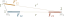
\includegraphics[scale=1.0]{figures/ch_02/fig_2_2.pdf}
		\caption[]{Uniaxial extension of a rod by an external force $F$: $1$ and $2$ are the schematic representation of adjacent atomic planes.}
		\label{fig:2_2}
	\end{center}
	\vspace{-0.7cm}
\end{figure}

The stresses a which appear in the extended rod will be
\begin{equation}\label{eq:2_5}
	\sigma = \frac{\ab{F}{int}}{S} = \frac{N}{S} \beta x = c x
\end{equation}

\noindent
where $c = N\beta/S$. Multiplying and dividing the right-hand side of \eqref{eq:2_5} by the distance between the atomic planes, $r_0$, we obtain
\begin{equation}\label{eq:2_6}
	\sigma = c r_0 \frac{x}{r_0} = E \varepsilon
\end{equation}

\noindent
where
\begin{equation}\label{eq:2_7}
	E = c r_0 = \frac{N}{S} \beta r_0
\end{equation}

\noindent
is termed the \textit{elasticity modulus,} or \textit{Young's modulus}, and
\begin{equation}\label{eq:2_8}
	\varepsilon = \frac{x}{r_0}
\end{equation}

\noindent
is the relative change in the lattice parameter in the direction of the external force $F$.

Multiplying the numerator and the denominator of \eqref{eq:2_8} by the number of atomic layers $N'$ contained in the sample of length $L$, we obtain
\begin{equation}\label{eq:2_9}
	\varepsilon = \frac{x N'}{r_0 N'} = \frac{\Delta{L}}{L}.
\end{equation}

\noindent
Hence, $\varepsilon$ is the relative elongation of the sample under the action of the external tensile load.

It follows from \eqn{2_6} that as long as the harmonic approximation remains valid, that is, as long as the forces acting between the particles displaced in relation to each other as a result of the deformation of the body remain linear functions of the displacement, the stresses $\sigma$ which appear in the body will remain proportional to the relative deformation of the body:
\begin{equation*}
	\sigma = E \varepsilon.
\end{equation*}

\noindent
The elasticity modulus $E$ serves as the proportionality factor.

Formula \eqref{eq:2_6} expresses the well-known \textit{Hooke's law}. It is valid only as long as the harmonic approximation is valid, that is, only for very small relative deformations $\varepsilon$.

The physical meaning of the elasticity modulus is quite evident from \eqn{2_6}. Putting $\varepsilon=1$, we find that $\sigma=E$. Hence, the elasticity modulus is numerically equal to the stress which is capable of causing an elongation $\Delta{L}=L$ of the sample, provided Hooke's law remains valid and the sample is not destroyed. No real material except rubber can stand such deformations.

Table \ref{table:2_1} shows the values of the elasticity modulus of some metallic crystals.

\begin{table}[!b]
	\renewcommand{\arraystretch}{1.2}
	\caption{}
	\vspace{-0.6cm}
	\label{table:2_1}
	\begin{center}\resizebox{0.84\linewidth}{!}{
			\begin{tabular}{lcccc}
				\toprule[1pt]
				\multirow{2}{*}{\textbf{Substance}} & \multicolumn{2}{c}{$E (\si{\giga\pascal})$} & \multicolumn{2}{c}{$G (\si{\giga\pascal})$}\\
				\cline{2-3} \cline{4-5}
				& \textbf{maximum} & \textbf{minimum} & \textbf{maximum} & \textbf{minimum}\\
				\midrule[0.5pt]\midrule[0.5pt]
				Aluminium	& $77$  & $64$  & $29$  & $25$\\
				Copper		& $194$ & $68$  & $77$  & $31$\\
				Iron		& $200$ & $135$ & $118$ & $60$\\
				Magnesium	& $514$ & $437$ & $184$ & $171$\\
				Tungsten	& $400$ & $400$ & $155$ & $155$\\
				Magnesium	& $126$ & $65$ & $497$ & $278$\\
				\bottomrule[1pt]
			\end{tabular}
	}\end{center}
\end{table}

It follows from data presented in Table \ref{table:2_1} that the elasticity modulus of solids is very large (of the order of \SIrange{e10}{e11}{\pascal}), which is an indication that the bonding forces in those bodies are very strong.

For some crystals the value of the elasticity modulus depends appreciably on the direction in which the lattice is deformed. Table \ref{table:2_1} shows the values of $E$ for directions in which it is at its minimum and at its maximum. For some crystals the ratio $\ab{E}{max}/\ab{E}{min}$ may be as high as $3$, pointing to a high degree of \textit{anisotropy} of such crystals.

The elasticity modulus depends only on the nature of the atoms (molecules) making up the body and on their mutual arrangement. It can be changed only by a substantial change in composition or internal structure of the solid. However, even in such cases the changes in $E$ are relatively small. Thus, high concentration alloying, heat treatment, cold rolling, etc. of steel result in great improvement in its hardness and in other mechanical properties but only in negligible (up to $10\%$) changes in its elasticity modulus; alloying copper with zinc up to $40\%$ leaves the elasticity modulus practically unchanged, although other properties experience a profound change.

We have discussed the tensile stress. However, all the considerations and the results obtained remain valid for other types of deformation---compression and shear---as well. In the latter case one should make use of the shear modulus $G$, whose values are also presented in Table \ref{table:2_1}.

When the external load is steadily increased, stress $\sigma$ and deformation $\varepsilon$ increase steadily too (\fig{2_3}). At some stress $\sigma_y$, characteristic of the specific crystal, the crystal is either destroyed or the direct proportionality between $\sigma$ and $\varepsilon$ ceases and a residual (plastic) deformation $\ab{\varepsilon}{res}$ sets in which remains after the external load has been removed. The first case is that of a brittle material and the second of a ductile one. The stress $\sigma_y$ at which a noticeable plastic flow in the body sets in is termed the \textit{yield stress} and $0$A and AB are the regions of the elastic and plastic deformations, respectively.

\begin{figure}[t]
	\begin{center}
		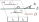
\includegraphics[scale=1.0]{figures/ch_02/fig_2_3.pdf}
		\caption[]{Typical extension curve of a ductile metal: $\sigma_y$ --- yield stress, $\ab{\varepsilon}{res}$ --- residual (plastic) deformation, $0$A---elastic deformation region, AB --- plastic deformation region.}
		\label{fig:2_3}
	\end{center}
	\vspace{-0.7cm}
\end{figure}

In brittle materials the elastic limit coincides with the tensile strength, and their destruction begins before a noticeable plastic flow sets in. In ductile metals, on the other hand, the elastic limit and the yield stress are, as a rule, much lower than the tensile strength, and these materials are destroyed only after a substantial plastic deformation has taken place.


\section{Principal laws governing plastic flow in crystals}\label{sec:14}

Residual deformations occur in all cases when the stress in ductile crystals tested for extension and compression exceeds the yield stress. However, neither extension nor compression can by themselves be the causes of such deformations. An increase in the length of the crystal can only result in an increase in the distance between the atomic planes perpendicular to the acting force. When these planes are drawn far enough apart, it may be that the forces of attraction shall no longer be able to compensate for the external load and the crystal will break. Compression can only draw the atomic planes closer together until the repulsive forces appearing between the atoms are able to counterbalance the external load. Deformation in this case is ideally elastic and cannot lead to irreversible displacement of parts of the lattice.

\begin{figure}[t]
	\begin{center}
		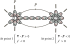
\includegraphics[scale=1.0]{figures/ch_02/fig_2_4.pdf}
		\caption[]{Crystal deformation by a shear force $\vec{F}$: (a) --- initial unstressed crystal; (b) --- elastic deformation caused by shearing stress not exceeding elastic limit; (c) --- early stages of plastic shear (slip) in the $S$ plane caused by stress exceeding elastic limit; (d) --- external force is removed, residual deformation (residual shift of one part of the lattice in relation to another) remains.}
		\label{fig:2_4}
	\end{center}
	\vspace{-0.7cm}
\end{figure}

Plastic deformation may only be the result of shearing stresses, which are able to shift some parts of the crystal in relation to the others without destroying the bonds between them. Such displacement is termed \textit{slipping}. It lies at the basis of the plastic flow process in crystalline materials. Figure \ref{fig:2_4} shows how residual deformations originate and develop in crystals [\fig{2_4}(a)] acted upon by a shearing force $\vec{F}$. As long as the elastic limit is not reached the crystal experiences elastic deformations [\fig{2_4}(b)] with the tangential stresses growing in proportion to the relative shearing deformation $\gamma$ (\textit{Hooke's law}):
\begin{equation}\label{eq:2_10}
	\tau = G \gamma
\end{equation}

\noindent
where $G$ is the shear modulus. After the crystal is relieved from external load the atoms return to their initial positions. When the elastic limit is exceeded, one part of the crystal shifts in relation to another [\fig{2_4}(c)] by one or more atomic distances along definite planes $S$ termed \textit{slip planes}. When the external load is withdrawn, the elastic stresses in the lattice vanish. However, one part of the crystal remains displaced in relation to another [\fig{2_4}(d)]. Such small irreversible displacements that proceed along numerous slip planes sum up to produce the residual deformation of the crystal as a whole.

The degree to which a crystal can be subjected to plastic deformations is determined, first of all, by the nature of the bonding forces acting between its structural elements.

The covalent bond with its rigorous directionality is appreciably weakened already by small relative displacements of the atoms. Shear destroys such bonds even before the atoms are able to establish them with other neighbouring atoms. On account of this the valence type crystals (such as diamond, silicon, germanium, antimony, bismuth, and arsenic) are incapable of plastic deformation. Outside the elastic deformation range they experience brittle destruction.

The metallic bond, which does not exhibit any directionality, on the other hand, remains practically unchanged as a result of relative tangential displacements of the atoms. This makes very great (some thousand atomic distances) relative displacements of some parts of the lattice possible, resulting in a high degree of ductility of crystals of this type.

The ionic bond occupies an intermediate position between the metallic and covalent bonds. It is less directional than the covalent bond but not so flexible as the metallic bond. Typical ionic crystals such as \ce{NaCl}, \ce{CaF2}, and \ce{KCl} are almost as brittle as the valence type crystals. At the same time silver chloride crystals are rather ductile.

Slipping takes place in crystals along definite crystallographic planes and directions, usually along the closest-packed planes and directions. This is because the closest-packed planes and directions are the strongest since the interatomic distances in them are the shortest and bonding is at its maximum. On the other hand, the distance between such planes is the greatest [see \eqref{eq:1_17}]; on account of this the bonding between them is at its minimum. Slipping along such planes and directions results in the minimum disarrangement in atomic order and is therefore the easiest to accomplish.

The combination of the slip plane and the slip direction, which lies in it, forms the \textit{slip system}. In the face-centered cubic lattice the slip plane coincides with the octahedral plane $(111)$ and the slip direction with the direction of the body diagonal $[111]$. In hexagonal crystals the $SS$ slip plane coincides with the base plane $(0001)$ and the $X$ slip direction with one of the three axes lying in the base plane (see \fig{2_5}, where $P$ is the external deforming load).

\begin{figure}[t]
	\begin{center}
		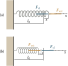
\includegraphics[scale=1.0]{figures/ch_02/fig_2_5.pdf}
		\caption[]{Slip planes and directions in a crystal.}
		\label{fig:2_5}
	\end{center}
	\vspace{-0.7cm}
\end{figure}

Numerous experiments have shown that the crystal begins to ``slip'' in the given slip system only after the shearing stress $\tau$ acting in this system reaches the critical value $\ab{\tau}{cr}$ termed the \textit{critical shearing stress}. Table \ref{table:2_2} shows the values of critical shearing stresses for some pure metallic single crystals.

\begin{table}[!b]
	\renewcommand{\arraystretch}{1.2}
	\caption{}
	\vspace{-0.6cm}
	\label{table:2_2}
	\begin{center}\resizebox{0.95\linewidth}{!}{
			\begin{tabular}{lcccc}
				\toprule[1pt]
				\textbf{Metal} & Impurity content $\parenthesis{\num{e-4}}$ & Slip plane & Slip direction & $\ab{\tau}{cr}$ $\parenthesis{\SI{e7}{\pascal}}$\\
				\midrule[0.5pt]\midrule[0.5pt]
				Cadmium	&	$0.40$	&	$(0001)$	&	$[100]$	&	$0.058$\\
				Copper	&	$10.0$	&	$(111)$		&	$[101]$	&	$0.100$\\
				Magnesium	&	$5.00$	&	$(0001)$	&	$[100]$	&	$0.083$\\
				Nickel	&	$20.0$	&	$(111)$		&	$[101]$	&	$0.580$\\
				Silver	&	$1.00$	&	$(111)$		&	$[101]$	&	$0.060$\\
				Zinc	&	$4.00$	&	$(0001)$	&	$[100]$	&	$0.094$\\
				\bottomrule[1pt]
			\end{tabular}
	}\end{center}
\end{table}

It follows from the data of \tab{2_2} that for the most ductile single crystals the critical shearing stress does not exceed \SI{e6}{\pascal}.

The critical shearing stress depends to a large extent on the prior deformation of the crystal rising with the increase in the latter. This phenomenon became known as strengthening, or \textit{cold working}. Thus a $350\%$ preliminary deformation of the magnesium single crystal increases $\ab{\tau}{cr}$ nearly $25$ times. Even greater is the effect of cold working on the cubic crystals---aluminium, copper, nickel, etc.

The strengthening of crystals is a witness to the fact that irreversible processes involving the relative displacement of atoms and of parts of the crystal take place. This results in changes of the internal energy of the crystals. Experimental study of this phenomenon has proved that the changes in the internal energy of solids in the process of their plastic deformation do, indeed, take place. Table \ref{table:2_3} shows the maximum amounts of energy that are accumulated by various metals in the process of their plastic deformation.

\begin{table}[!b]
	\renewcommand{\arraystretch}{1.2}
	\caption{}
	\vspace{-0.6cm}
	\label{table:2_3}
	\begin{center}\resizebox{0.34\linewidth}{!}{
			\begin{tabular}{lc}
				\toprule[1pt]
				\textbf{Metal} & $Q \parenthesis{\si{\joule\per\kilo\gram}}$\\
				\midrule[0.5pt]\midrule[0.5pt]
				Aluminium	&	$4400$\\
				Brass		&	$2000$\\
				Copper 		&	$2000$\\
				Iron		&	$4800$\\
				Nickel		&	$3120$\\
				\bottomrule[1pt]
			\end{tabular}
	}\end{center}
\end{table}

Should this energy be transformed into heat it would suffice to heat the metal by several degrees.

Since the accumulation of energy in the crystal in the process of its plastic deformation involves irreversible displacements of the atoms and of parts of the crystal, this energy is, in effect, the energy of \textit{residual stresses} remaining in elastically deformed parts of the crystal lattice.

Because of a higher value of internal energy in a cold worked crystal it is less thermodynamically stable than the annealed crystal. This gives rise to processes that tend to bring the crystal to the equilibrium state. Relaxation and recrystallization are two such processes.

\textit{Relaxation} consists in the dissipation of internal stresses, with the atoms of the deformed parts of the lattice returning to their regular positions. This process does not involve visible changes in the crystal structure and results in a partial or complete removal of the strengthening obtained as a result of plastic deformation. Being a diffusion-controlled process relaxation proceeds at a rate that strongly depends on temperature and on the latent heat of defect formation. Metals with a low melting point (such as tin, lead, cadmium, zinc) have comparatively high self-diffusion rates already at room temperatures. Accordingly, their relaxation rates at room temperatures are quite noticeable. At the same time there is practically no relaxation at room temperature in the metals with a high melting point; but the relaxation rate rises sharply as the temperature is increased (the relaxation process goes as far in $1$ minute at \SI{315}{\degreeCelsius} as it would in a hundred years at room temperature).

Another process that also results in the disappearance of the hardening in a cold worked crystal---the \textit{recrystallization} process---proceeds intensely at temperatures of the order of one quarter of the melting temperature of the metal (on the absolute scale). In contrast to relaxation, which produces no visible changes in the crystal structure, recrystallization involves nucleation and growth of new crystals free from internal stresses. The nucleation of such crystals takes place in the first instance in the most deformed parts of the lattice, where much of the excess free energy is concentrated. In this way, a complete change in the microscopic structure of the crystal takes place with the crystal generally going over from the single state to the polycrystalline one. In the process of recrystallization the latent heat accumulated in the deformed crystal is given off in the form of heat.

\section{Mechanical twinning}\label{sec:15}

Plastic deformation may also take the form of \textit{twinning}, which is a process of step-by-step relative displacement of atomic planes parallel to the twinning plane by a fixed distance equal to a fraction of the lattice parameter. Figure \ref{fig:2_6} shows the diagram of twinning of the crystal AECDA. The area ABCDA is the undeformed part of the crystal, BECB is the part where twinning has taken place, and BC is the \textit{twinning axis}. The positions of atoms before twinning are denoted by crosses. The plane passing through the twinning axis and separating the region of twinning from the undeformed part of the crystal is termed \textit{twinning plane}.

\begin{figure}[t]
	\begin{center}
		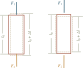
\includegraphics[scale=1.0]{figures/ch_02/fig_2_6.pdf}
		\caption[]{Twinning in a crystal: sign ``$+$'' denotes initial atomic positions in the twinning region.}
		\label{fig:2_6}
	\end{center}
	\vspace{-0.7cm}
\end{figure}

Figure \ref{fig:2_6} shows that twinning results in the displacement of the atoms of the plane $11$ relative to the twinning plane BC by a fraction of interatomic distance in the twinning direction. The plane $22$ is displaced relative to the plane $11$ by the same fraction of interatomic distance, the displacement relative to the twinning plane being twice as great. In other words, every atomic plane parallel to the twinning plane is displaced in itself by a distance proportional to its distance from the twinning plane. As a result, the atoms in the twinned region assume positions that are mirror reflections of the positions in the undeformed part of the crystal in the twinning plane.

Twinning, in the same way as slipping, may take place only along specific crystallographic planes. In case of a face-centered cubic crystal this is the $(112)$ plane, in case of a hexagonal close-packed crystal this is the $(1012)$ plane, etc. For twinning to take place the tangential stresses should exceed some critical value. The process is a very rapid one and is usually accompanied by a characteristic crackle.

Because only negligible relative displacements of the neighbouring atomic planes are involved in the process of twinning it cannot result in a great residual deformation. For instance, a complete transition of a zinc crystal to the twinned form brings about only a $7.39\%$ elongation. For this reason in crystals capable of plastic flow by means of slipping, twinning is responsible only for a negligible fraction of the total plastic deformation. In contrast to that, negligible deformation that precedes destruction of the valence crystals, in which slipping cannot take place, is due to twinning. In hexagonal crystals unfavourably oriented in relation to the external force twinning and subsequent reorientation of the crystal may result in appreciable residual deformations produced by the normal slipping process.

\section{Theoretical and real shear strengths of crystals}\label{sec:16}

Shear is the principle mechanism of plastic flow in crystals. For a long time it was presumed that such shear takes place by means of a rigid displacement of one part of the crystal in relation to another simultaneously along the entire slip plane $SS$ (\fig{2_7}).

Let us make a rough estimate of the tangential stress needed to produce such shear.

\begin{figure}[t]
	\begin{minipage}[t]{0.52\linewidth}
		\begin{center}
			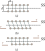
\includegraphics[scale=1]{figures/ch_02/fig_2_7.pdf}
			\caption[]{Diagram of rigid shear: (a) --- equilibrium position of atoms in atomic planes adjoining the slip plane; (b) --- gradual shift of one plane in relation to another caused by external stress $\tau$; (c) --- lower atomic plane as a whole displaced by one interatomic distance in relation to the upper plane.}
			\label{fig:2_7}
		\end{center}
	\end{minipage}
	\hfill{ }%\hspace{-0.1cm}
	\begin{minipage}[t]{0.43\linewidth}
		\begin{center}
			
\includegraphics[scale=1]{figures/ch_02/fig_2_8.pdf}
			\caption[]{Variation of resistance to shear in the process of displacement of one part of the lattice in relation to another.}
			\label{fig:2_8}
		\end{center}
	\end{minipage}
\vspace{-0.3cm}
\end{figure}

The atoms of two adjacent parallel planes in an undeformed lattice occupy equilibrium sites corresponding to the minimum of the potential energy [\fig{2_7}(a)]. The forces acting between them are zero. As one atomic plane is displaced relative to the other tangential stresses $\tau$ appear. They resist the shear and tend to bring back the original equilibrium state [\fig{2_7}(b)]. If we assume the dependence of those stresses on the displacement to be sinusoidal (\fig{2_8}), we shall be able to express the resistance to shear in the form
\begin{equation}\label{eq:2_11}
	\tau = A \sin\parenthesis{\frac{2\pi x}{b}}
\end{equation}

\noindent
where $x$ is the displacement of the atoms from their equilibrium positions, $b=a$ the interatomic distance in the slip plane, and $A$ is a constant. For small displacements $\sin(2\pi x/b)\approx 2\pi x/b$ and therefore
\begin{equation}\label{eq:2_12}
	\tau = A \parenthesis{\frac{2\pi x}{b}}.
\end{equation}

On the other hand, for small displacements Hooke's law is valid:
\begin{equation}\label{eq:2_13}
	\tau = G \frac{x}{d}
\end{equation}

\noindent
where $G$ is the shear modulus, and $d$ the distance between the planes. From \eqref{eq:2_12} and \eqref{eq:2_13} we obtain $A=(b/d)(G/2\pi)$. Therefore
\begin{equation}\label{eq:2_14}
	\tau = \frac{b}{d} \frac{G}{2\pi} \sin\parenthesis{\frac{2\pi x}{b}}.
\end{equation}

The maximum Value $\ab{\tau}{cr}$ of the tangential stress $\tau$ is attained for $x=b/4$ and this is assumed to be the theoretical strength:
\begin{equation}\label{eq:2_15}
	\ab{\tau}{cr} = \frac{b}{d} \frac{G}{2\pi}.
\end{equation}

\noindent
Setting $b=d$, we obtain
\begin{equation}\label{eq:2_16}
	\ab{\tau}{cr} = \frac{G}{2\pi}.
\end{equation}

Hence, the critical shearing stress should be equal to about one tenth of the shear modulus. A more rigorous consideration of the nature of the bonding forces acting between the atoms leads to a negligible correction factor. The minimum value that was obtained for $\ab{\tau}{cr}$ is $G/30$. Table \ref{table:2_4} shows experimental and theoretical values of $\ab{\tau}{cr}$ for several metals.

\begin{table}[!b]
	\renewcommand{\arraystretch}{1.2}
	\caption{}
	\vspace{-0.6cm}
	\label{table:2_4}
	\begin{center}\resizebox{0.83\linewidth}{!}{
			\begin{tabular}{lcccc}
				\toprule[1pt]
				\multirow{2}{*}{\textbf{Metal}} & $\ab{\tau}{cr} \parenthesis{\SI{e7}{\pascal}}$, & \multirow{2}{*}{$G \parenthesis{\SI{e7}{\pascal}}$} & \multicolumn{2}{c}{$\ab{\tau}{cr} \parenthesis{\SI{e7}{\pascal}}$, \textbf{theory}}\\
				\cline{4-5}
				& \textbf{experiment} & & $G/(2\pi)$ & $G/30$ \\
				\midrule[0.5pt]\midrule[0.5pt]
				Cadmium & $0.06$ & $2640$ & $420$ & $88$\\
				Copper & $0.10$ & $4620$ & $735$ & $154$\\
				Iron & $2.90$ & $6900$ & $1100$ & $230$\\
				Magnesium & $0.08$ & $1770$ & $280$ & $59$\\
				Nickel & $0.58$ & $7800$ & $1240$ & $260$\\
				Silver & $0.06$ & $2910$ & $459$ & $97$\\
				Zinc & $0.09$ & $3780$ & $600$ & $126$\\
				\bottomrule[1pt]
			\end{tabular}
	}\end{center}
\end{table}

A comparison of these figures shows that the real shear strength of crystals is some $3$-$4$ orders of magnitude less than the theoretical value. This points to the fact that shear in crystals does not take place by means of a rigid relative displacement of atomic planes but by means of a mechanism involving the displacement of a comparatively small number of atoms at a time. The understanding of this fact led to the evolution of the dislocation theory of plastic flow of crystals.

\section{The dislocation concept. Principal types of dislocations}\label{sec:17}

The dislocation theory of plastic flow assumes that the slipping process starts always at imperfections in the crystal structure and develops along the shear plane by means of a gradual motion of this imperfection which at a time involves only a limited number of atoms. Such imperfections are termed \textit{dislocations}.

\textbf{Edge dislocations.} Suppose gliding took place in the crystal K in the plane ABCD in the direction of the vector $\vec{b}$ involving the area AHED (\fig{2_9}). The atomic planes on both sides from the slip plane AHED are displaced in relation to one another by the distance $b$ in the slip direction. The boundary HE separating the area AHED, where slipping took place, from the area HBCE, where slipping has not yet taken place, constitutes an edge dislocation and the vector $\vec{b}$ is termed the \textit{Burgers vector}. It describes how far slipping has proceeded in the area AHED.

\begin{figure}[t]
	\begin{minipage}[t]{0.45\linewidth}
		\begin{center}
			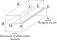
\includegraphics[scale=0.9]{figures/ch_02/fig_2_9.pdf}
			\caption[]{Shear that creates an edge dislocation. Shear took place only in region AHED of slip plane ABCD. Boundary HE is the edge dislocation.}
			\label{fig:2_9}
		\end{center}
	\end{minipage}
	\hfill{ }%\hspace{-0.1cm}
	\begin{minipage}[t]{0.51\linewidth}
		\begin{center}
			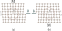
\includegraphics[scale=0.95]{figures/ch_02/fig_2_10.pdf}
			\caption[]{Arrangement of atoms in the plane perpendicular to dislocation line HE (see \fig{2_9}). Dislocation occupies the region in which lattice atoms are displaced from their equilibrium sites (bounded by a circle): $0$ --- dislocation centre; (a) --- positive dislocation; (b) negative dislocation.}
			\label{fig:2_10}
		\end{center}
	\end{minipage}
\vspace{-0.3cm}
\end{figure}

Figure \ref{fig:2_10} shows the arrangement of atoms in a plane perpendicular to the dislocation line. As a result of the shift which took place over the area AHED the upper part of the lattice contains one atomic plane (plane OM) more than the lower. Because of that the atomic row $1$ lying above the shear plane contains one atom more than the row $2$ below this plane. The interatomic distances in the upper row near the point $0$ (the dislocation centre) will accordingly be shorter than the normal value (the lattice is contracted), while the interatomic distances in the lower row near the point $0$ will be longer (the lattice is extended). As the distance to the left or to the right, and up or down, from the dislocation centre $0$ increases, the deformation of the lattice gradually subsides and at an appropriate distance from $0$ in the crystal normal disposition of atoms is restored. However, in the direction perpendicular to the plane of the diagram the dislocation passes through the entire crystal or through a considerable part of it.

Thus, a feature of the edge dislocation is the existence of an ``excess'' atomic plane OM in some part of the crystal. Therefore the process of formation of such a dislocation may be imagined as that of pulling the lattice apart and inserting an additional atomic plane in it. Such plane is termed \textit{extra plane}. If the plane is inserted into the upper part of the lattice, the edge dislocation is assumed to be positive [\fig{2_10}(a)]. But if the extra plane is inserted into the lower part of the lattice, the dislocation is assumed to be negative [\fig{2_10}(b)]. A dislocation whose Burgers vector is equal to the lattice parameter is called the \textit{unit dislocation}. When a unit dislocation passes through a cross section of the crystal, one part of it shifts in relation to the other by a distance $b$. The motion of a positive dislocation to the left causes the same shift of parts of the lattice as a motion of a negative dislocation to the right [\fig{2_10}(a,b)].

\begin{figure}[t]
	\begin{center}
		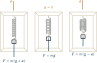
\includegraphics[scale=1.1]{figures/ch_02/fig_2_11.pdf}
		\caption[]{Formation of a screw dislocation: (a) --- shear which produces the screw dislocation. It took place in the ABCD plane. Boundary AD is a screw dislocation; (b) --- arrangement of atoms around the screw dislocation. Plane of drawing is parallel to slip plane. White circles denote atoms of the plane lying immediately above the slip plane, black circles denote atoms of the plane lying under the slip plane.}
		\label{fig:2_11}
	\end{center}
	\vspace{-0.7cm}
\end{figure}

\textbf{Screw dislocations.} Suppose an incomplete unit shift is made in the crystal K in the direction of the vector $\vec{b}$ over the area ABCD, as shown in \fig{2_11}(a); AD is the boundary of the area that experienced the shift. In \fig{2_11}(b) the white circles denote the atoms of the plane immediately above the slip plane and black circles the atoms of the plane below the slip plane. In the undeformed part of the crystal to the left of AD the atoms of those planes are arranged one on top of the other; therefore the black circles coincide with the white (this is shown by white circles with circles in the centre). In the right-hand part of the crystal, where the shift has covered one interatomic distance, that is, to the right of EH, the atoms of the planes discussed above are also arranged one on top of the other. However, in the narrow strip ADEH the atoms of the upper plane are displaced in relation to those of the lower plane the more the farther away they are from the boundary AD. This displacement results in a local deformation of the lattice, which became known as the \textit{screw dislocation}; the boundary AD is termed \textit{dislocation axis}. The origin of the term screw dislocation may be easily understood from \fig{2_12}: the motion of the atom ``a'' towards the atoms ``b, c, d, e'', etc. [\fig{2_12}(a)] lying in the plane of the screw dislocation proceeds, as may be seen from \fig{2_12}(b), along a spiral. A distinction is made between right and left screw dislocations (\fig{2_13}); the motion of both in opposite directions results in a shift in one direction.

\begin{figure}[t]
	\begin{minipage}[t]{0.5\linewidth}
		\begin{center}
			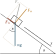
\includegraphics[scale=0.9]{figures/ch_02/fig_2_12.pdf}
			\caption[]{Explaining the origin of the ``screw dislocation'': (a) --- arrangement of atoms in a screw dislocation; (b) --- atom ``a'' moves towards atoms ``b, c, d, e'', etc. constituting the screw dislocation along a spiral.}
			\label{fig:2_12}
		\end{center}
	\end{minipage}
	\hfill{ }%\hspace{-0.1cm}
	\begin{minipage}[t]{0.46\linewidth}
		\begin{center}
			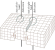
\includegraphics[scale=0.9]{figures/ch_02/fig_2_13.pdf}
			\caption[]{Arrangement of atoms in the plane perpendicular to dislocation line HE (see \fig{2_9}). Dislocation occupies the region in which lattice atoms are displaced from their equilibrium sites (bounded by a circle): $0$ --- dislocation centre; (a) --- positive dislocation; (b) negative dislocation.}
			\label{fig:2_13}
		\end{center}
	\end{minipage}
\vspace{-0.3cm}
\end{figure}

Comparing Figures \ref{fig:2_9} and \ref{fig:2_11}(a), we see that in contrast to the edge dislocation, which is perpendicular to the Burgers vector $\vec{b}$, the screw dislocation is parallel to it. The motion of the edge dislocation is in the direction of the Burgers vector $\vec{b}$, and the motion of the screw dislocation is in the direction perpendicular to it.

Recently, experimental methods for direct observation of dislocations have been developed. Figure \ref{fig:2_14}(a) shows a schematic diagram of an electron micrograph of a thin film of platinum phthalocyanine and \fig{2_14}(b,c) an electron micrograph of a copper sulphide crystal obtained with the aid of a special procedure. Dark stripes on the micrographs are the traces of the atomic planes, which in platinum phthalocyanine are arranged at a distance of \SI{12}{\angstrom} from one another and in copper sulphide at a distance of \SI{1.88}{\angstrom}. The
micrographs distinctly show the extra planes which terminate inside the crystal and form edge dislocations.

Figure \ref{fig:2_14}(d) shows an optical micrograph of a decorated screw dislocation in a \ce{CaF2} crystal. The method of decoration as used for transparent crystals consists in the precipitation along their dislocation cores of impurity atoms, which make the dislocation visible in an optical microscope. The striking agreement between those pictures and the theoretical concepts as set out in Figures \ref{fig:2_10} and \ref{fig:2_12} is worthy of admiration. Points of exit of dislocations on the crystal surface may be detected with the aid of etching. When a crystal is etched in a specially selected etch, the parts of the crystal where the lattice is most deformed dissolve more readily because the atoms in those parts possess an excess energy and are chemically more active. The places of exit of dislocations on the crystal surface are just such parts. Figure \ref{fig:2_15} shows a photograph of an etched germanium surface. The dark patches are the points of exit of dislocations.

\begin{figure}[t]
	\begin{minipage}[t]{0.62\linewidth}
		\begin{center}
			\includegraphics[scale=0.8]{figures/ch_02/fig_2_14.pdf}
			\caption[]{Observation of dislocations in an electron microscope: (a) --- schematic diagram of an electron micrograph of a thin platinum phthalocyanine film (dark lines are atomic traces); (b), (c) --- electron micrograph of a copper sulfide crystal (dark lines are traces of atomic planes); (d) --- screw dislocation in a \ce{CaF2} crystal obtained by decoration method.}
			\label{fig:2_14}
		\end{center}
	\end{minipage}
	\hfill{ }%\hspace{-0.1cm}
	\begin{minipage}[t]{0.34\linewidth}
		\begin{center}
			\includegraphics[scale=0.8]{figures/ch_02/fig_2_15.pdf}
			\caption[]{Etch pits on germanium surface. Dark points along the grain boundary are points of exit of dislocations.}
			\label{fig:2_15}
		\end{center}
	\end{minipage}
\vspace{-0.3cm}
\end{figure}

\section{Forces needed to move dislocations}\label{sec:18}

Suppose there is a positive dislocation with the centre at $0$, bounded at points ``a'' and ``k'' and lying in the plane $S$ in which slipping is possible [\fig{2_16}(a)]. In equilibrium the force with which the lattice acts on the dislocation is zero. This may easily be seen from the roller model shown in \fig{2_17}. The structure of the upper row of rollers which normally occupy recesses between the rollers of the lower row was deformed so that the section AB which previously contained $6$ rollers now contains only $5$. Such deformation gives rise to forces which tend to return the rollers $1, 2, 4, 5$ to their stable equilibrium positions (the forces $\vec{F}_1, \vec{F}_2, \vec{F}_3, \vec{F}_4, \vec{F}_5$). The forces applied to rollers $7, 5$ and $2, 4$ are equal in magnitude and opposite in direction.
Therefore, if the rollers of the upper row are interconnected by means of an elastic spring acting as a bond between them, the forces $\vec{F}_1$ and $\vec{F}_5, \vec{F}_2, \vec{F}_4$ will be mutually compensated and the system will be in a state of equilibrium.

\begin{figure}[t]
	\begin{center}
		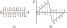
\includegraphics[scale=1.2]{figures/ch_02/fig_2_16.pdf}
		\caption[]{Calculating the force needed to move a dislocation: (a) --- region of positive dislocation in crystal; $0$ is dislocation centre, ``a'' and ``k'' are dislocation boundaries, $S$ is the slip plane; (b) --- forces needed to move an atom in the dislocation region (forces applied to atoms equidistant from the dislocation centre are equal in magnitude and opposite in direction).}
		\label{fig:2_16}
	\end{center}
	\vspace{-0.7cm}
\end{figure}
\begin{figure}[t]
	\begin{center}
		\includegraphics[scale=1.0]{figures/ch_02/fig_2_17.pdf}
		\caption[]{Roller model of an edge dislocation. Forces applied to ``atoms'' $1, 5$ and $2, 4$ are equal in magnitude and opposite in direction.}
		\label{fig:2_17}
	\end{center}
	\vspace{-0.7cm}
\end{figure}

The same situation occurs in the case of a dislocation schematically shown in \fig{2_16}(b); the forces acting on atoms of the upper row occupying positions symmetrical with respect of the dislocation centre $0$ are equal in magnitude but opposite in direction (the forces $F_b=F_j, F_c=F_i, F_d=F_h, F_e=F_g$). Therefore the resultant force is zero and the dislocation is in a state of equilibrium. If, however, the dislocation moves a little in the slip plane the symmetrical arrangement of the atoms in respect of the dislocation centre will be disturbed giving rise to a force which resists the motion of the dislocation. It is evident from \fig{2_17} that this force cannot be great since the movement of the rollers $1$ and $2$ to their new equilibrium position is to a large extent the result of the action of the forces excercised on them by the rollers $4$ and $5$, which also strive to occupy positions of stable equilibrium. Calculations show the tangential stress needed to move the dislocation to be equal to
\begin{equation}\label{eq:2_17}
	\tau_0 = \frac{2G}{(1-\nu)} \exp\bracket{-\frac{2\pi b}{d(1-\nu)}}
\end{equation}

\noindent
where $G$ is the shear modulus, $\nu$ the Poisson ratio, $b$ the interatomic distance, and $d$ the distance between adjacent slip planes. The stress $\tau_0$ is the theoretical value of the critical shearing stress. Setting $b=d$ and $\nu=0.3$, we obtain $\tau_0=\num{3e-4}\,G$. Within an order of magnitude this coincides with the experimental values of $\ab{\tau}{cr}$. Thus, the theory of dislocations resolves the contradiction between the theoretical and the experimental values of shear strength of crystals.

The mechanism of motion by means of dislocations is quite frequent in nature. Snakes, worms, and shellfish move, because they generate dislocations. The motion of an earth-worm begins with the formation of an ``extension'' dislocation near the neck. The dislocation subsequently spreads along the body to the tail [\fig{2_18}(a)]. In contrast, the motion of most snakes involves the formation of a ``contraction'' dislocation near the tail and its motion towards the head [\fig{2_18}(b)].

\begin{figure}[t]
	\begin{center}
		\includegraphics[scale=1.0]{figures/ch_02/fig_2_18.pdf}
		\caption[]{Dislocation mechanism of motion of (a) an earth-worm and (b) a snake.}
		\label{fig:2_18}
	\end{center}
	\vspace{-0.7cm}
\end{figure}

\section{Sources of dislocations. Strengthening of crystals}\label{sec:19}

The dislocations in a real crystal are formed in the process of its growth from the melt or from a solution. Figure \ref{fig:2_19}(a) shows the boundaries of two blocks growing towards each other. The blocks make a small angle $\varphi$ between themselves. As the blocks fuse together, some of the atomic planes do not spread through the entire crystal but terminate at block boundaries. Those are the places where dislocations are formed [\fig{2_19}(b)]. The same situation occurs in the process of fusion of differently oriented grains in a polycrystalline sample. Since the block and grain boundaries in real solids are very extensive, the number of dislocations in them is enormous---as many as \num{e12} dislocations per square metre can be counted in well annealed metals. After cold working (rolling, drawing, etc.) dislocation densities rise to \SIrange{e15}{e16}{\per\metre\squared}. Those dislocations accumulate almost the entire energy absorbed by the metal in the process of plastic deformation.

Vacancy clusters may also serve as sources of dislocations in an undeformed crystal. Figure \ref{fig:2_20} shows an example of the formation of a positive and a negative dislocation from a cluster of vacancies.

\begin{figure}[t]
	\begin{minipage}[t]{0.51\linewidth}
		\begin{center}
			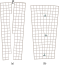
\includegraphics[scale=1]{figures/ch_02/fig_2_19.pdf}
			\caption[]{Formation of dislocations at block boundaries: (a) --- two blocks growing towards each other at an angle $\varphi$; (b) --- dislocations appearing when the blocks fuse together.}
			\label{fig:2_19}
		\end{center}
	\end{minipage}
	\hfill{ }%\hspace{-0.1cm}
	\begin{minipage}[t]{0.44\linewidth}
		\begin{center}
			\includegraphics[scale=1]{figures/ch_02/fig_2_20v.pdf}
			\caption[]{Dislocations formed from vacancy clusters: (a) --- vacancy cluster in crystal; (b) --- positive and negative dislocations formed from this cluster.}
			\label{fig:2_20}
		\end{center}
	\end{minipage}
\vspace{-0.3cm}
\end{figure}

The shear process in a crystal in response to an applied external force is, in effect, the motion of dislocations in the slip planes and their emergence through the crystal surface. Should only the dislocations already present in the crystal be responsible for this process, plastic deformation would lead to their exhaustion and to the perfection of the crystal. This is in contradiction with experience, which demonstrates that as deformation grows the lattice does not become more perfect. In fact, just the opposite is true: the density of dislocations grows in the process. It is an established fact that dislocations responsible for plastic deformation are generated in the shear process itself by the action of the external force applied to the crystal. One such generation mechanism was discovered in 1950 by F. C. Frank and W. T. Read. For the purpose of better understanding this mechanism let us consider soap bubble formation with the aid of a tube (\fig{2_21}). After the end of the tube has been immersed in a soap solution a flat film remains that closes the tube's orifice. As the air pressure in the tube is increased, the film swells and passes through the stages $1, 2, 3, 4$, etc. Until it assumes the shape of a hemisphere (stage $3$) its state is unstable: as pressure falls the film contracts striving to return to the original state $1$. After the bubble has passed stage $3$ the state of the bubble changes: it is now capable of evolution not only at a constant but also at a gradually decreasing pressure until it leaves the end of the tube. After the first bubble the second begins to be formed, followed by the third, etc.

\begin{figure}[t]
	\begin{center}
		\includegraphics[scale=1]{figures/ch_02/fig_2_21.pdf}
		\caption[]{Process of formation of a soap bubble.}
		\label{fig:2_21}
	\end{center}
	\vspace{-0.7cm}
\end{figure}

Now let us discuss the operation of the Frank-Read source. Figure \ref{fig:2_22}(a) shows an edge dislocation $DD'$ in a slip plane; points $D$ and $D'$ are fixed and do not take part in the motion of the dislocation. Dislocations may be anchored at the points of intersection with other dislocations, at impurity atoms, etc. Under the action of an external stress $\tau$ the dislocation starts bending in the same way as was the case with the soap film and at some time assumes the shape of a semicircle [\fig{2_22}(b)]. Just like the soap film the dislocation can continue to bend only if $\tau$ grows steadily until it assumes the shape of a semicircle. Its subsequent evolution takes place by itself and results in the formation of two loops [\fig{2_22}(c)], which after meeting at point C [\fig{2_22}(d)] divide the dislocation in two: an external one, which closes forming an external circle [\fig{2_22}(e)], and an internal one, which returns to the original position $DD'$. The external dislocation grows until it reaches the surface of the crystal and results in an elementary shift; the internal dislocation having returned to the initial position $DD'$ begins again to bend under the action of the applied force and to grow in the manner described above. Such process may be repeated any number of times eventually leading to a noticeable shift of one part of the crystal in relation to another in a particular slip plane.

\begin{figure}[t]
	\begin{center}
		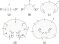
\includegraphics[scale=1.1]{figures/ch_02/fig_2_22.pdf}
		\caption[]{Operating sequence of a Frank-Read source: (a) --- initial position of dislocation $DD'$, (b) --- acted upon by external force the dislocation bends and assumes the shape of a semicircle; (c), (d) --- further symmetric development of the dislocation loop; (e) --- formation of external closed dislocation loop spreading across the crystal and of internal dislocation $DD'$ returning to the original position.}
		\label{fig:2_22}
	\end{center}
	\vspace{-0.7cm}
\end{figure}

Low shear strength of crystals is due to the presence of innate dislocations and to the generation of others in the process of Shear. On the other hand, it is an established fact that the crystal is strengthened in the process of plastic deformation accompanied by the growth in the number of defects. The essence of such strengthening is the interaction of dislocations with each other and with other types of lattice defects causing their motion in the lattice to be obstructed.

\textbf{Interaction of dislocations.} Every dislocation, being the cause of elastic stresses of the lattice, creates a force field around itself which may be described by the values of the tangential $\tau$ and normal $\sigma$ stresses at every point. When another dislocation enters this field, forces begin to act which strive to bring the dislocations together or to move them apart. Dislocations of like signs lying in one plane are repelled, while those of opposite signs are attracted. This is the reason why, as dislocations are accumulated in a definite plane, the crystal's resistance to shear is increased and the crystal is strengthened.

\textbf{Surmounting of obstacles.} Suppose a dislocation when moving in a slip plane under the action of tangential stresses $\tau$ runs into a stationary obstacle D, for instance, an intersection with some other dislocation, an impurity atom, or some other type of defect. Figure \ref{fig:2_23} shows the method by means of which dislocation AB could, theoretically, surmount obstacle D: as the dislocation approaches D (positions $1, 2, 3$) it gradually bends forming a loop that envelops the obstacle. Behind the obstacle the loop closes and the dislocation A$'$B$'$ again becomes a straight line. Figure \ref{fig:2_24} shows a photograph illustrating a case when a dislocation runs into a stationary obstacle (dark lines represent dislocations decorated by etching). The similarity in the pictures leaves not a trace of doubt as to the validity of the theoretical pattern shown in \fig{2_23}.

\begin{figure}[t]
	\begin{minipage}[t]{0.631\linewidth}
		\begin{center}
			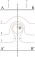
\includegraphics[scale=1]{figures/ch_02/fig_2_23.pdf}
			\caption[]{Schematic representation of an edge dislocation surmounting an obstacle: AB --- shape of edge dislocation away from the obstacle D; $1, 2, 3$ --- gradual bending of the dislocation as it approaches D and closing of the newly formed loop behind the obstacle; A$'$B$'$ --- straightening of the dislocation far away from the obstacle.}
			\label{fig:2_23}
		\end{center}
	\end{minipage}
	\hfill{ }%\hspace{-0.1cm}
	\begin{minipage}[t]{0.33\linewidth}
		\begin{center}
			\includegraphics[scale=0.98]{figures/ch_02/fig_2_24.pdf}
			\caption[]{Microphotographs of a chromium grain. Dark lines are etched dislocations ($\times 2000$).}
			\label{fig:2_24}
		\end{center}
	\end{minipage}
\vspace{-0.3cm}
\end{figure}

In passing around the obstacle, the length of the dislocation and the deformation of the lattice are increased, which requires additional work to be performed. Therefore, the resistance to the motion of the dislocation in the interval where it has to surmount a defect is much greater than in other parts of the lattice. This is the essence of the fact that defects strengthen a crystal. The growth in the number of dislocations in the crystal with greater plastic deformation increases the number of obstacles at points of their intersection, which is the cause of strengthening brought about by plastic deformation. Impurity atoms have a similar effect: they create local lattice imperfections and thereby hinder the motion of the dislocations, with the result that the crystal's resistance to shear is increased. Block and grain boundaries and foreign inclusions in the lattice are especially effective in hindering the motion of the dislocations. They sharply increase the resistance to the motion of dislocations and greater stresses are required to overcome their effect. The phenomenon of strengthening in the process of cold working, in the process of introducing impurity atoms (doping), and in the process of formation of inclusions (tempering, aging, etc.) is widely used in practice to improve mechanical properties of engineering materials. This method enabled the strength of the materials to be increased from $6$ to $8$ times in the last 40 years.

\section{Brittle strength of solids}\label{sec:20}

The destruction of solids may be of one of two principal types: of the \textit{brittle} and of the \textit{plastic}, or \textit{viscous}, types.

Brittle destruction takes place if the tensile strength of the material is below the elastic limit. Such a material experiences only elastic deformation prior to destruction. No irreversible changes take place in such a material before it breaks down.

In the ductile materials the elastic limit is not only below the tensile strength but also below the yield stress. Because of that the destruction process is preceded by an appreciable plastic deformation, which prepares the subsequent destruction process. In this case strength, being a typical kinetic parameter, is strongly dependent on the time the destructive stress is applied.

To begin with, let us discuss brittle strength of solids.

\textbf{Theoretical strength of solids.} There have been numerous attempts to calculate the strength of solids on the basis of molecular
interaction in them. The strength $\sigma_0$ thus calculated is termed
\textit{theoretical strength}.

Here is a glance at some of the methods of estimating $\sigma_0$.

\textit{Polanyi's method}. The simplest method of estimating the strength of solids theoretically is due to M. Polanyi. Its essence is as follows.

\begin{figure}[t]
	\begin{center}
		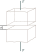
\includegraphics[scale=1.0]{figures/ch_02/fig_2_25.pdf}
		\caption[]{Calculating theoretical strength of solids after Polanyi (explanation in text).}
		\label{fig:2_25}
	\end{center}
	\vspace{-0.7cm}
\end{figure}

Suppose a tensile stress $\sigma$ is applied to a rod of a cross-sectional area of \SI{1}{\metre\squared} (\fig{2_25}). This stress increases the distance between the atomic planes. It is assumed that for destruction to take place a stress $\sigma_0$ able to increase the distance between the atomic planes by a value of the order of the lattice parameter $a$ should be applied. The work needed to move an atomic plane a distance $a$ away from the neighbouring plane is assumed to be equal to $\sigma_0 a$. It is further assumed that this work is transformed into the free energy of two new surfaces with a total area of \SI{2}{\metre\squared} formed as a result of the breakup, the free energy being equal to $2\alpha$, where $\alpha$ is the surface energy (``surface tension'') of the solid. Hence,
\begin{equation*}
	\sigma_0 a = 2 \alpha
\end{equation*}

\noindent
and the theoretical strength is
\begin{equation}\label{eq:2_18}
	\sigma_0 = \frac{2 \alpha}{a}.
\end{equation}

\noindent
For copper $\alpha\approx\SI{1.7}{\joule\per\metre\squared}$, $a=\SI{3.6e-10}{\metre}$, and $\sigma_0\approx\SI{e10}{\pascal}$, for silver $\alpha\approx\SI{1.14}{\joule\per\metre\squared}$, $a=\SI{4e-10}{\metre}$, and $\sigma_0=\SI{0.6e10}{\pascal}$.

\textit{Determination of $\sigma_0$ from the heat of sublimation}. The energy equal to the heat of sublimation $\ab{Q}{s}$ is required for the evaporation of a mole of a solid. For the evaporation of one molecular layer of the area of \SI{1}{\metre\squared} the required energy $W$ is a fraction of $\ab{Q}{s}$ equal to the ratio of the mass of this layer $m$ to the molar mass $M$:
\begin{equation*}
	W = \frac{\ab{Q}{s}}{m}.
\end{equation*}

\noindent
But
\begin{equation*}
	m = \ab{N}{s} \mu,\quad M = \ab{N}{A} \mu
\end{equation*}

\noindent
where $\mu$ is the molecular weight, $\ab{N}{A}=\SI{6.023e23}{\per\mole}$ the Avogadro number, and $\ab{N}{s}$ the number of molecules per square metre of the solid's surface.

For an intermolecular distance of $a$ the area per molecule is approximately equal to $a^2$ and the number of molecules per square metre
$\ab{N}{S}\approx a^2$. Therefore,
\begin{equation*}
	W = \ab{Q}{s} \frac{\ab{N}{s}}{\ab{N}{A}} \approx \frac{\ab{Q}{s}}{\ab{N}{A} a^2}.
\end{equation*}

Should the assumption be made that the evaporating molecules loose contact with the solid's surface when they are a distance of the order of the lattice parameter $a$ away from it, we would obtain for the force needed to tear away an entire surface layer as a whole
\begin{equation}\label{eq:2_19}
	\sigma_0 \approx \frac{W}{a} = \frac{\ab{Q}{s}}{\ab{N}{A}} \frac{1}{a^2}
\end{equation}

\noindent
$\sigma_0$ is assumed to be the theoretical strength of the solid.

For copper $\ab{Q}{s}=\SI{3e5}{\joule\per\mole}, a=\SI{3.6e-10}{\metre}, and \sigma_0\approx\SI{e10}{\pascal}$. Similar calculations lead to the following results: for iron $\sigma_0\approx\SI{2.3e10}{\pascal}$, for aluminium $\sigma_0\approx\SI{0.6e10}{\pascal}$, and for silver $\sigma_0\approx\SI{0.6e10}{\pascal}$.

\textit{Calculating $\sigma_0$ from the forces of molecular interaction.} Finally, let us discuss the method of calculating theoretical strength of solids from the forces of molecular interaction. Figure \ref{fig:2_26} shows the dependence of the potential energy $U(x)$ and the force of interaction between the particles $f(x)$ on the distance $x$ between them. Since it is not easy to determine the exact law governing $f(x)$, the practice is to approximate this dependence by various functions. For instance, M. Polanyi and E. Orowan used the approximation in the form of a half of a sinusoid:
\begin{equation}\label{eq:2_20}
	f(x) = \ab{f}{max} \sin\parenthesis{\frac{2\pi x}{c}}.
\end{equation}

\begin{figure}[t]
	\begin{center}
		\includegraphics[scale=1.0]{figures/ch_02/fig_2_26.pdf}
		\caption[]{Calculating theoretical strength from forces of molecular interaction (explanation in text).}
		\label{fig:2_26}
	\end{center}
	\vspace{-0.7cm}
\end{figure}

\noindent
When a body of cross-sectional area of \SI{1}{\metre\squared} is slowly torn in two, the required force is $\sigma=f\ab{N}{s}$, where $\ab{N}{s}$ is the number of particles per square metre of the cross section. Substituting $f$ from \eqref{eq:2_20} we obtain
\begin{equation}\label{eq:2_21}
	\sigma = \sigma_0 \sin\parenthesis{\frac{2\pi x}{c}}
\end{equation}

\noindent
where $\sigma_0=\ab{f}{max}\ab{N}{s}$ is the theoretical strength of the body.

For small displacements relation \eqref{eq:2_21} may be rewritten in the form
\begin{equation*}
	\sigma = \frac{\sigma_0 2\pi x}{c}.
\end{equation*}

\noindent
On the other hand, for small displacements Hooke's law is valid:
\begin{equation*}
	\sigma = \frac{E x}{c}.
\end{equation*}

Equating the right-hand sides of these equations, we obtain
\begin{equation}\label{eq:2_22}
	\sigma_0 \approx \frac{E}{2\pi} \approx 0.1 E.
\end{equation}

Calculations show that a more accurate estimate of the nature of the bonding in solids results only in a negligible correction to \eqref{eq:2_22}.

Comparing the values of theoretical strength $\sigma_0$ calculated with the aid of various methods we see that all of them yield nearly the same result whose order of magnitude is $0.1E$. Therefore it may be legitimately assumed that
\begin{equation}\label{eq:2_23}
	\sigma_0 \approx 0.1 E.
\end{equation}

\noindent
This is an enormous figure of the order of \SIrange{e9}{e10}{\pascal}.

\textbf{Real (technical) strength of solids.} The strength of real crystals and solids used for technical purposes is termed \textit{real}, or \textit{technical}, \textit{strength} $\ab{\sigma}{r}$. Table \ref{table:2_5} shows the values of the elasticity modulus $E$, of theoretical strength $\sigma_0\approx 0.1E$, of technical strength $\ab{\sigma}{r}$, and of the ratio $\sigma_0/\ab{\sigma}{r}$ for some industrial materials.

\begin{table}[!b]
	\renewcommand{\arraystretch}{1.2}
	\caption{}
	\vspace{-0.6cm}
	\label{table:2_5}
	\begin{center}\resizebox{0.98\linewidth}{!}{
			\begin{tabular}{lcccc}
				\toprule[1pt]
				\multirow{2}{*}{\textbf{Substance}} &  \textbf{Elasticity modulus} & \textbf{Theoretical strength} & \textbf{Technical strength} & \multirow{2}{*}{$\sigma_0/\ab{\sigma}{r}$}\\
				& $E\,\parenthesis{\SI{e7}{\pascal}}$ & $\sigma_0\approx 0.1E \parenthesis{\SI{e7}{\pascal}}$ & $\ab{\sigma}{r} \parenthesis{\SI{e7}{\pascal}}$ & \\
				\midrule[0.5pt]\midrule[0.5pt]
				Aluminium & $6000$ & $600$ & $9.0$ & $65$\\
				Copper & $12000$ & $1200$ & $23$ & $50$\\
				Glass & $8000$ & $800$ & $8.0$ & $100$\\
				Iron & $21000$ & $2100$ & $30$ & $70$\\
				Rock salt & $4000$ & $400$ & $0.5$ & $800$\\
				Silver & $8000$ & $800$ & $18$ & $45$\\
				\bottomrule[1pt]
			\end{tabular}
	}\end{center}
\end{table}

It follows from the data of \tab{2_5} that the technical strength of solids is from $2$ to $3$ orders of magnitude less than their theoretical
strength.

At present there is a general agreement that such discrepancy between $\sigma_0$ and $\ab{\sigma}{r}$ is due to the presence of defects in real solids of various types, in particular of microscopic cracks which reduce the strength of solids. This is accounted for by the so-called \textit{Griffith theory}. Let us calculate the technical strength using this theory.

We take a sample in the form of a thin plate and apply a tensile stress $\sigma$ to it [\fig{2_27}(a)]. The density of elastic energy in such an elastically extended sample is $\sigma^2/(2E)$\footnote{Indeed, the relative deformation in a sample under stress a is $\varepsilon=\sigma/E$, the absolute deformation $\Delta{L}=\varepsilon L$ ($L$ being the length of the sample). The work performed by the stress $\sigma$ to extend the sample by $\Delta{L}$ is $(1/2)\sigma S\Delta{L}=\sigma^2SL/(2E)=\sigma^2V/(2E)$ ($S$ is the cross-sectional area and $V$ the volume of the sample). This work is transformed into the elastic energy of the sample of volume $V$. Therefore, the specific volume density of the elastic energy is $\sigma^2/(2E)$.}.

Now let us imagine that a transverse microscopic crack of the length $l$ running through the entire thickness $\delta$ of the sample has developed in it. The appearance of the crack is accompanied by the formation of a free surface $S\approx 2l\delta$ inside the sample and by an increase in the sample's energy by the amount $\Delta{U}_1\approx 2l\delta\alpha$ ($\alpha$ is the free surface energy of the sample per unit area). On the other hand, the formation of a crack relieves the elastic stress from the volume $V\approx l^2\delta$ of the sample, whereby its elastic energy is reduced by the amount $\Delta{U}_2\approx l^2\delta\sigma^2/(2E)$. The total change in the energy of the sample $W(l)$ brought about by the appearance of a crack in it is
\begin{equation}\label{eq:2_24}
	W(l) = 2 l \delta \alpha - l^2 \delta \frac{\sigma^2}{2E}.
\end{equation}

Figure \ref{fig:2_27}(b) shows the dependence of $W$ on the length $l$ of the crack. It has a maximum where its derivative vanishes: $\diffin{W}{l}=2\delta\alpha-l\delta\sigma^2/E$. Denote the length of the crack corresponding to the maximum energy by $\ab{l}{cr}$. We obtain from the last relation
\begin{equation}\label{eq:2_25}
	\ab{l}{cr} = \frac{2 \alpha E}{\sigma^2}.
\end{equation}

\begin{figure}[t]
	\begin{center}
		\includegraphics[scale=1.0]{figures/ch_02/fig_2_27.pdf}
		\caption[]{The Griffith theory of calculating the real strength of solids (explanation in text).}
		\label{fig:2_27}
	\end{center}
	\vspace{-0.7cm}
\end{figure}

It may be seen from \fig{2_27}(b) that as long as the length $l$ of the crack remains below the critical value $\ab{l}{cr}$, energy is needed for it to develop. On the other hand, starting with $l=\ab{l}{cr}$ further extension of the sample results in a reduction in its energy. Therefore, it takes place spontaneously with the brittle destruction of the sample as the final result.

Hence, the technical strength of solids having microscopic cracks should be calculated according to the Griffith theory from relation \eqref{eq:2_25}:
\begin{equation}\label{eq:2_26}
	\ab{\sigma}{r} \approx \parenthesis{\frac{2\alpha E}{l}}^{1/2} \approx \beta \parenthesis{\frac{\alpha E}{l}}^{1/2}.
\end{equation}

\noindent
This result was subsequently verified by many investigators for various quite different methods of applying loads to the sample. A negligible difference was observed only in case of the numerical coefficient $\beta$.

Should we substitute the values of $\alpha, E, \ab{\sigma}{r}$ for copper ($\alpha\approx\SI{1.7}{\joule\per\metre\squared}, E=\SI{1.2e11}{\pascal}, \ab{\sigma}{r}=\SI{1.8e8}{\pascal}$) into \eqref{eq:2_26}, we would obtain $l\approx\SI{8e-6}{\metre}$. Approximately the same values of $l$ may be obtained for other solids.

It follows that for the strength of the solids to be reduced from the theoretical value to the value of the technical strength microscopic cracks of the order of several micrometers in length should develop in them up to the moment preceding their destruction. Many factors may be the cause of such cracks.

The cracks may be produced in the course of the production of the solid, especially in the course of its mechanical processing. A proof of this is, in particular, a significant dependence of the strength of the sample on its dimensions, especially in the small dimensions range. Thus the strength of a glass filament of \SI{2.5}{\micro\metre} in diameter is almost $100$ times that of a massive sample. The explanation is that as the dimensions of the sample are reduced so too is the probability of a large crack responsible for low strength appearing in it. Such dependence of the strength on the dimensions of the sample became known as the \textit{scale factor}. The cracks may be the result of a large number of vacancies merging together.

Figure \ref{fig:2_28} shows a dislocation mechanism of crack production. Dislocations of a similar sign move in slip plane SS and meeting obstacle B begin to accumulate in its vicinity. Large stresses able to produce cracks $l$ may develop at the head of this dislocation pile-up.

\begin{figure}[t]
	\begin{center}
		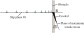
\includegraphics[scale=1.0]{figures/ch_02/fig_2_28.pdf}
		\caption[]{Formation of a crack near a dislocation pile-up.}
		\label{fig:2_28}
	\end{center}
	\vspace{-0.7cm}
\end{figure}

\section{Time dependence of fhe strength of solids}\label{sec:21}

The theory of strength based on the condition \eqref{eq:2_26} and discussed above describes actually the final stage of the destructive process when the body already contains cracks able to cause brittle rupture.

However, the initial stages of the destructive process during which the cracks originate and grow to attain critical dimensions $\ab{l}{cr}$ are also important. This process is a gradual one and takes time $\tau$ to be completed. The time $\tau$ that it takes for the destructive process to develop from the moment the load is applied to the body to the moment
of rupture is termed the \textit{durability} of the material.

The firsts experiments aimed at investigating durability were carried out by S. N. Zhurkov and G. M. Bartenev with coworkers. They also developed modern notions about the physical nature of durability.

It was established by experiments that the durability $\tau$, the tensile stress $\sigma$, and the absolute temperature $T$ are related by the expression:
\begin{equation}\label{eq:2_27}
	\tau = \tau_0 e^{(U_0 - \gamma\sigma)/(\ab{k}{B} T)}
\end{equation}

\noindent
where $\tau_0, U_0$, and $\gamma$ are constants dependent on the nature and structure of the body.

For $T = $constant, formula \eqref{eq:2_27} may be rewritten in the form
\begin{equation}\label{eq:2_28}
	\tau = A e^{-\beta\sigma}
\end{equation}

\noindent
where $A=\tau_0 e^{U_0/(\ab{k}{B} T)}$, and $\beta=\gamma/(\ab{k}{B} T)$.

Formulae \eqref{eq:2_27} and \eqref{eq:2_28} were tested on a great number of different materials (metals, polymers, haloid compounds, etc.) in an $8$ to $10$ order of magnitude range of the values of $\tau$ and in a wide range of the values of $T$.

\begin{figure}[t]
	\begin{center}
		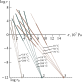
\includegraphics[scale=1.0]{figures/ch_02/fig_2_29.pdf}
		\caption[]{Durability versus stress for aluminium ($1$), Plexiglas ($2$), and silver chloride ($3$).}
		\label{fig:2_29}
	\end{center}
	\vspace{-0.7cm}
\end{figure}

Figure \ref{fig:2_29} shows the dependence of the durabilities $\tau$ of aluminium ($1$), Plexiglas ($2$), and silver chloride ($3$) on the applied stress $\sigma$ at various temperatures expressed in the $\log{\tau}$ versus $\sigma$ coordinate system. It may be seen from \fig{2_29} that the dependence $\tau(\sigma)$ in semilogarithmic coordinates is well represented by a straight line. A family of such straight lines obtained for a given material at different temperatures resembles a fan with the apex at some point called pole.
It follows from \eqn{2_27} that $\tau$ will be independent of $T$ and that the straight lines $\log{\tau(\sigma)}$ at different temperatures will intersect at one point (at the pole) only if $U_0-\gamma\sigma=0$; but in that case $\log{\tau}=\log{\tau_0}$. Hence, the pole should be at a distance $\log{\tau_0}$ below the $\sigma$-axis.

It is evident from \fig{2_29} that the poles for all the materials tested lie practically on the same straight line parallel to the $\sigma$-axis. This means that $\tau_0$ is approximately the same for all the materials. Experiments show it to be of the order of \SIrange{e-12}{e-13}{\second}, that is, close to the period of oscillations of atoms in solids.

Let us take the logarithm of \eqref{eq:2_27}:
\begin{equation}\label{eq:2_29}
	\log{\tau} = \log{\tau_0} + \frac{(U_0 - \gamma\sigma)}{\ab{k}{B}T} = \log{\tau_0} + \frac{U}{\ab{k}{B}T},\quad U = U_0 - \gamma\sigma.
\end{equation}

\noindent
Measuring the dependence of $\log{\tau}$ on $1/T$ for constant values of $\sigma$, we can determine $U$ for various values of the stress $\sigma$ experimentally; the dimensions of $U$ are that of energy and because of this it is termed \textit{activation energy of the destructive process}. Figure \ref{fig:2_30} shows the dependence of the activation energy of rupture of viscose fibre on stress for various temperatures.
It may be seen that $U$ is independent of $T$ and is determined solely by $\sigma$; for $\sigma=0$ the maximum value of $U$ is $U_0\approx\SI{40}{\kilo\cal\per\mole}$; for a stress $\sigma\approx\SI{107e7}{\pascal}$ we see that $U=0$.
Figure \ref{fig:2_31} shows that for $\sigma\approx\SI{107e7}{\pascal}$ a practically instantaneous rupture of viscous fibre takes place (during the time $\tau_0$), no matter what its temperature is.

\begin{figure}[t]
	\begin{minipage}[t]{0.48\linewidth}
		\begin{center}
			\includegraphics[scale=1]{figures/ch_02/fig_2_30.pdf}
			\caption[]{Activation energy of rupture of viscose fibre at different temperatures (triangles, $-\SI{76}{\degreeCelsius}$; circles, $+\SI{20}{\degreeCelsius}$; crosses, $+\SI{80}{\degreeCelsius}$) versus stress.}
			\label{fig:2_30}
		\end{center}
	\end{minipage}
	\hfill{ }%\hspace{-0.1cm}
	\begin{minipage}[t]{0.48\linewidth}
		\begin{center}
			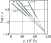
\includegraphics[scale=1]{figures/ch_02/fig_2_31.pdf}
			\caption[]{Durability of viscose fibre at different temperatures versus stress.}
			\label{fig:2_31}
		\end{center}
	\end{minipage}
\vspace{-0.3cm}
\end{figure}

Meticulous experiments carried out by S. N. Zhurkov with coworkers and by other investigators on a variety of materials demonstrated that for metals $U_0$ is quite close to the sublimation energy $\ab{Q}{s}$ and for polymers to the thermal destruction energy $\ab{Q}{d}$. Table \ref{table:2_6} shows the values of $U_0, \ab{Q}{s}$, and $\ab{Q}{d}$ for some materials. It may be seen that $U_0$ coincides either with $\ab{Q}{s}$ or with $\ab{Q}{d}$ with a high degree of accuracy.

\begin{table}[!b]
	\renewcommand{\arraystretch}{1.2}
	\caption{}
	\vspace{-0.6cm}
	\label{table:2_6}
	\begin{center}\resizebox{0.98\linewidth}{!}{
			\begin{tabular}{lccc}
				\toprule[1pt]
				\multirow{2}{*}{\textbf{Substance}} &  \textbf{Activation energy of} & \textbf{Sublimation energy} & \textbf{Thermal destruction} \\
				& \textbf{destruction}, $U_0\,\parenthesis{\SI{e5}{\joule\per\mole}}$ & $\ab{Q}{s}\,\parenthesis{\SI{e5}{\joule\per\mole}}$ & \textbf{energy}, $\ab{Q}{d} \parenthesis{\SI{e5}{\joule\per\mole}}$\\
				\midrule[0.5pt]\midrule[0.5pt]
				Aluminium & $2.16$ & $2.2$ & \\
				Nickel & $3.48$ & $3.4$ & \\
				Nylon & $1.8$ & & $1.72$\\
				Platinum & $4.8$ & $5.1$ & \\
				Polymethyl methacrylate & $2.16$ & & $2.1$-$2.2$\\
				Polyvinyl chloride & $1.4$ & & $1.28$\\
				Silver & $2.56$ & $2.72$ & \\
				Teflon & $3.0$ & & $3.0$-$3.1$\\
				Zinc & $1.0$ & $1.08$ & \\
				\bottomrule[1pt]
			\end{tabular}
	}\end{center}
\end{table}

Universal validity of the dependence thus obtained merits the conclusion that the process of destruction of a solid is one of a kinetic nature (that is, develops in time) and its origin is the same for all solids. Modern notions of the physical mechanism of this process are set out below.

The atoms in a solid take part in thermal oscillations with a period of $\tau_0 \approx$ \SIrange{e-12}{e-13}{\second}. Thermal fluctuations from time to time result in the rupture of chemical bonds. The probability of this process depends on the height of the potential barrier of destruction $U$ and on the temperature $T$. This probability increases with the rise in $T$ and the decrease in $U$. In the absence of external stress $\sigma$ the energy required to break a bond is equal to the energy of the bond itself. This is the reason why the height of the potential barrier $U_0$ obtained from experiments in mechanical destruction of solids turned out to be equal to the sublimation heat of metals and to the thermal destruction energy of polymers.

The stresses induced in a body reduce the height of the potential barrier from $U_0$ to $U_0-\gamma\sigma$ and thus increase the probability of rupture of the bonds and, consequently, the number of ruptured bonds per unit volume.

The formation of submicroscopic volumes in which the bonds have been broken and their merging results eventually in the nucleation and development of cracks. When the length of the cracks attains a critical value, the body breaks up under the applied stress. The higher is the stress a the lower the activation barrier $U_0-\gamma\sigma$ and the greater the rate of bond rupture; therefore it takes less time for the destructive process to develop, that is the less should be the durability
of the body. This is exactly what is observed in practice.

From the above point of view the destruction of solids should take place at any stresses provided the time they act is long enough. But in that case it is not easy to understand why bridges and other installations built many centuries ago and carrying loads all that time still remain intact.

To explain this fact we again turn to \fig{2_29}. We see that the lower the temperature the weaker the load dependence of durability is. This dependence is practically nill at sufficiently low temperatures. For glasses and metals with a high melting point already room temperatures are low enough. Because of that their strength is actually a unique characteristic of the material. In all other conditions it is not justified to speak of strength without mentioning the time during which the material is to work under load. Thus, industrial products made of Plexiglas during a year's service can endure loads not exceeding $30\%$ of their short-time strength; steam turbine blades working at high temperatures are calculated for strength always with account taken of their durability.

\section{Methods of increasing the strength of solids}\label{sec:22}

The nucleation mechanism of breaks in continuity and the mechanism of crack growth are both greatly influenced by the atomic structure of solids. Therefore, strength is a structure-sensitive characteristic of such bodies.

Stresses in crystals occasion the production of dislocations and their motion in slip planes. In this way, plastic shifts resulting in plastic deformations are realized. Meeting impurities, grain and block boundaries, interceptions of slip planes, etc., the dislocations lose their mobility and the crystal is hardened. As was mentioned above, stresses may develop at the head of a dislocation pile-up capable of causing cracks.

To increase the strength of such bodies it is necessary to retard the production of dislocations and the nucleation and growth of cracks.

This can be done by two methods.

(1) By producing imperfection-free crystals free from internal stress sources, which in the long run cause the nucleation of cracks.

This method has up to the present been realized only in the filament type crystals known by the name of ``whiskers''. They are single crystals grown under special conditions using the method of decomposition or reduction of appropriate chemical compounds, the method of condensation of vapours of pure metals at an appropriate temperature in hydrogen or in an inert gas, and the method of electroplating metals from a solution onto electrodes of extremely small dimensions. The filament-type crystals are usually \SIrange{2}{10}{\milli\metre} long and \SIrange{5}{50}{\micro\metre} thick.

A striking property of such crystals is that their mechanical parameters are extremely high. Their strength turned out to be close to the theoretical strength of solids. Thus, the strength of iron whiskers is about \SI{1.34e10}{\pascal}, of copper whiskers about \SI{3e9}{\pascal}, and of zinc whiskers \SI{2.3e9}{\pascal}, while the strength of normal samples made from those metals is \SI{3e8}{\pascal}, \SI{2e8}{\pascal}, and \SI{1.8e8}{\pascal}, respectively.

Filament-type crystals of iron experience only elastic deformation reaching an enormous figure of the order of $5\%$-$6\%$, after which brittle destruction occurs. Note that in normal iron noticeable plastic flow starts already at a deformation of $\varepsilon\approx 0.01\%$.

The unusually high mechanical parameters of the filament crystals are due to their ideal internal structure. Such crystals contain practically no dislocations, are exceptionally pure and their surface is so perfect that even a magnification of $40000$ times fails to reveal any traces of roughness. Such perfection is mainly due to the condition of growth of small-size crystals, in which the freezing-in of lattice imperfections is less probable because it is easier for them to leave the crystal through a nearby surface.

Because of the absence of dislocations and of other defects in filament crystals a shift in a slip plane can only take the form of a rigid shift, in which the bonds of all the atoms in the slip plane are simultaneously broken. Stresses close to the theoretical stress limit of the crystals are needed to effect such a shift and this is what is observed in practice.

An unnaturally great elastic deformation of the whiskers is due to the absence of mobile dislocations, which in normal crystals are responsible for the plastic deformations occurring already at very low stresses.

Hence, the first method, the method of producing imperfection-free (in particular, dislocation-free) crystals, holds out a promise of producing materials of extreme strength close to the theoretical strength of solids.

(2) The second method is a direct opposite of the first. It consists in the maximum deformation of the internal structure of a crystal through the introduction of impurities, precipitation of dispersed phases, great plastic deformation, etc. Such defects hinder the motion of the dislocations and the growth of cracks and thus increase the strength of the material, as was already discussed in detail above. Science and industry have up to now made use only of this method and succeeded in attaining with it a strength of the order of \SI{4e9}{\pascal}. The effect this had on technology may be inferred from the following example. The specific weight of a modern aircraft engine is about $1$ kgf per hp; at the turn of the century it was about $250$ kgf per hp.

The recent times have witnessed the appearance of composite materials consisting of a matrix filled with filament crystals. Stainless steel, nickel, titanium and other materials are used for the matrix. The matrices are filled with tungsten, aluminium oxide, etc. filaments. The results obtained so far hold out a promise of obtaining by this method in the near future materials of $5$ to $10$ times the strength (especially at elevated temperatures) of the best steels and of $1.5$-$2$ times lighter weight.

The strength of amorphous bodies and glass polymers is no less sensitive to internal structure. The strength of glass and quartz filaments newly extruded at a high temperature and practically free from defects\footnote{Since the atomic structure of amorphous bodies is irregular, the term defect may apply only to inclusions (clusters of foreign atoms, cracks, inhomogeneities) large if compared with atomic dimensions.} is $100$ times as high as that of normal specimens and quite close to the theoretical value.

The room temperature strength of unoriented glass polymers is of the order of \SI{e8}{\pascal}. Films and fibres made of them having an oriented structure have a strength of the order of \SI{e9}{\pascal} comparable to that of high quality steels. With a perfect orientation of the polymer molecule chain the strength of the needlelike crystals of the polymer may be as high as \SI{3e10}{\pascal}. If one takes into account that the density of the polymers is close to unity, one can imagine how great their value for technology may be.

There is a rapidly growing demand on the quality of the materials for modern science and technology. Already now there is a need for materials able to withstand temperatures of several thousand degrees with the necessary strength characteristics at such temperatures and without any noticeable plastic deformation at normal loads.

What are the prospects for such materials?

One of the feasible methods for producing such extra strong and extra heat-resistant materials was proposed by the Soviet physicist A. V. Stepanov who pointed to a particular property of such molecular crystals as sulfur. The crystal of sulfur is constructed of molecules bonded by relatively weak molecular forces. Because of that the strength of the crystal and its melting point are low (\SI{115}{\degreeCelsius}). The atoms in the sulfur molecule itself, on the other hand, are held together by powerful chemical bonds. If one would be able to construct a sulfur lattice with the atoms retaining the same bonds that act in the molecule, the result would be an extremely strong crystal with the melting point of about \SI{34700}{\degreeCelsius}. Similar modifications could be introduced into other molecular crystals as well. Are there any real grounds for such projects? The fact that we were able to transform soft graphite and hexagonal boron nitride into extra strong, hard, and high melting point diamond and borazon crystals by substituting powerful covalent bonds for weak van der Waals forces lends ground to such hopes. The prospects that will be opened by such materials are so enormous that any work, no matter how great, put into their production shall be generously rewarded.
